\usetikzlibrary{arrows.meta, positioning, decorations.pathreplacing}

% ---------------------------------------------------------------
% Colors
% ---------------------------------------------------------------
\definecolor{activegray}{RGB}{120,120,120}   % CPU busy checking / waking up
\definecolor{reactgray}{RGB}{60,60,60}       % CPU reacting to the event
\definecolor{eventyellow}{RGB}{255,193,7}    % event lightning bolt

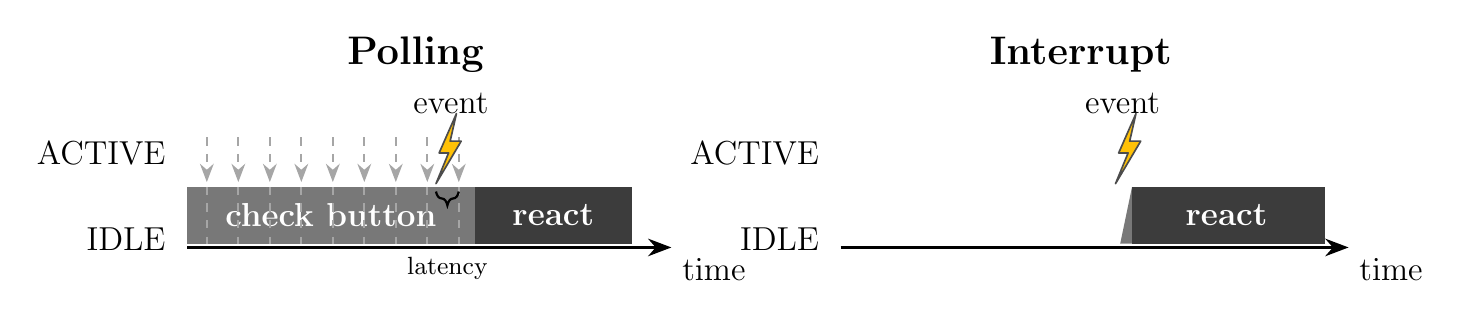
\begin{tikzpicture}[
    font=\sffamily,
    >=Stealth
]

% ============================================================
% Global dimensions
% ============================================================
\def\axisW{5.8}
\def\barH{0.72}
\def\baseline{0}

% ============================================================
% LEFT: POLLING
% ============================================================
\begin{scope}[xshift=0cm]

    % Panel title
    \node[anchor=south, font=\bfseries\Large] at (2.9,2.05) {Polling};

    % Labels
    \node[anchor=east, font=\large] at (-0.15,1.15) {ACTIVE};
    \node[anchor=east, font=\large] at (-0.15,0.05) {IDLE};

    % CPU activity
    \fill[activegray] (0,0) rectangle (3.65,\barH);
    \fill[reactgray]  (3.65,0) rectangle (5.65,\barH);

    % Text inside blocks
    \node[text=white, font=\bfseries\large] at (1.825,0.36) {check button};
    \node[text=white, font=\bfseries\large] at (4.65,0.36) {react};

    % Polling checks
    \foreach \x in {0.25,0.65,1.05,1.45,1.85,2.25,2.65,3.05,3.45} {
        \draw[dashed, -{Stealth}, line width=0.8pt, gray!70]
            (\x,1.35) -- (\x,0.78);
            \draw[dashed, line width=0.8pt, gray!70]
            (\x,\barH) -- (\x,0);
    }

    % Event label
    \node[font=\large] at (3.35,1.78) {event};

    % Lightning bolt
    \fill[eventyellow, draw=black!70, line width=0.6pt, line join=round]
        (3.42,1.65) -- (3.20,1.15) -- (3.32,1.15) -- (3.16,0.76)
        -- (3.48,1.30) -- (3.34,1.30) -- cycle;

    % Detection-latency bracket
    \draw[decorate, decoration={brace, amplitude=5pt, mirror},
          line width=0.8pt] (3.16,0.66) -- (3.45,0.66)
          node[midway, below=20pt, font=\small] {latency};

    % Time axis
    \draw[->, line width=1.2pt] (0,-0.05) -- (6.15,-0.05)
        node[below right, font=\large] {time};

\end{scope}

% ============================================================
% RIGHT: INTERRUPT
% ============================================================
\begin{scope}[xshift=8.3cm]

    % Panel title
    \node[anchor=south, font=\bfseries\Large] at (3.05,2.05) {Interrupt};

    % Labels
    \node[anchor=east, font=\large] at (-0.15,1.15) {ACTIVE};
    \node[anchor=east, font=\large] at (-0.15,0.05) {IDLE};

    % Wake-up transition
    \fill[activegray] (3.55,0) -- (3.7,\barH) -- (3.7,0) -- cycle;

    % Reaction
    \fill[reactgray] (3.7,0) rectangle (6.15,\barH);
    \node[text=white, font=\bfseries\large] at (4.9,0.36) {react};

    % Event label
    \node[font=\large] at (3.58,1.78) {event};

    % Lightning bolt
    \fill[eventyellow, draw=black!70, line width=0.6pt, line join=round]
        (3.75,1.65) -- (3.53,1.15) -- (3.65,1.15) -- (3.49,0.76)
        -- (3.81,1.30) -- (3.67,1.30) -- cycle;


    % Time axis
    \draw[->, line width=1.2pt] (0,-0.05) -- (6.45,-0.05)
        node[below right, font=\large] {time};
\end{scope}

\end{tikzpicture}